\documentclass{article}

\usepackage{amsmath}
\usepackage[capitalise]{cleveref}
\usepackage[a4paper, margin=1in]{geometry}
\usepackage{graphicx}
\usepackage{mathtools}
\usepackage{parskip}
\usepackage{titling}

\setlength{\droptitle}{-5em}

\makeatletter
\newcommand{\shorteq}{%
  \settowidth{\@tempdima}{-}% Width of hyphen
  \,\resizebox{\@tempdima}{\height}{=}\,%
}
\makeatother

\title{Cosmology Homework}
\author{Calvin Sykes}
\date{\today}

\begin{document}
\maketitle

{\large {\bfseries Question 1}}

$a)$ The {\bf comoving distance} $d_x$ is given by:
\begin{align}
  d_x(z)&=\frac{c}{H_0}\int_0^z\frac{\mathrm{d}z'}{E(z')},\label{eq:1a}\\
  \shortintertext{where}
  E(z)&=\left[\Omega_m(1+z)^3+\Omega_\Lambda\right]^{1/2}\nonumber
\end{align}

$b)$ The {\bf angular diameter distance} $d_A$ is given by:
\begin{equation}
  d_A(z)=\frac{d_x(z)}{1+z}\label{eq:1b}
\end{equation}

$c)$ The {\bf luminosity distance} $d_L$ is given by:
\begin{equation}
  d_L(z)=(1+z)^2 d_A(z)\label{eq:1c}
\end{equation}

$d)$ The {\bf age of the Universe} $t$ is given by:
\begin{equation}
  t(z)=\frac{1}{H_0}\int_z^\infty\frac{\mathrm{d}z'}{(1+z')E(z')}\label{eq:1d}
\end{equation}

\Cref{eq:1a,eq:1b,eq:1c,eq:1d} are plotted for $\left\{z \mid 0\leq z \leq 10\right\}$ in \cref{fig:q1} below. Since these equations only depend on $h$ via the prefactor $1/H_0$, this term may be factored out to give results independent of the value of $h$.

\begin{figure}[hb]
  \centering
  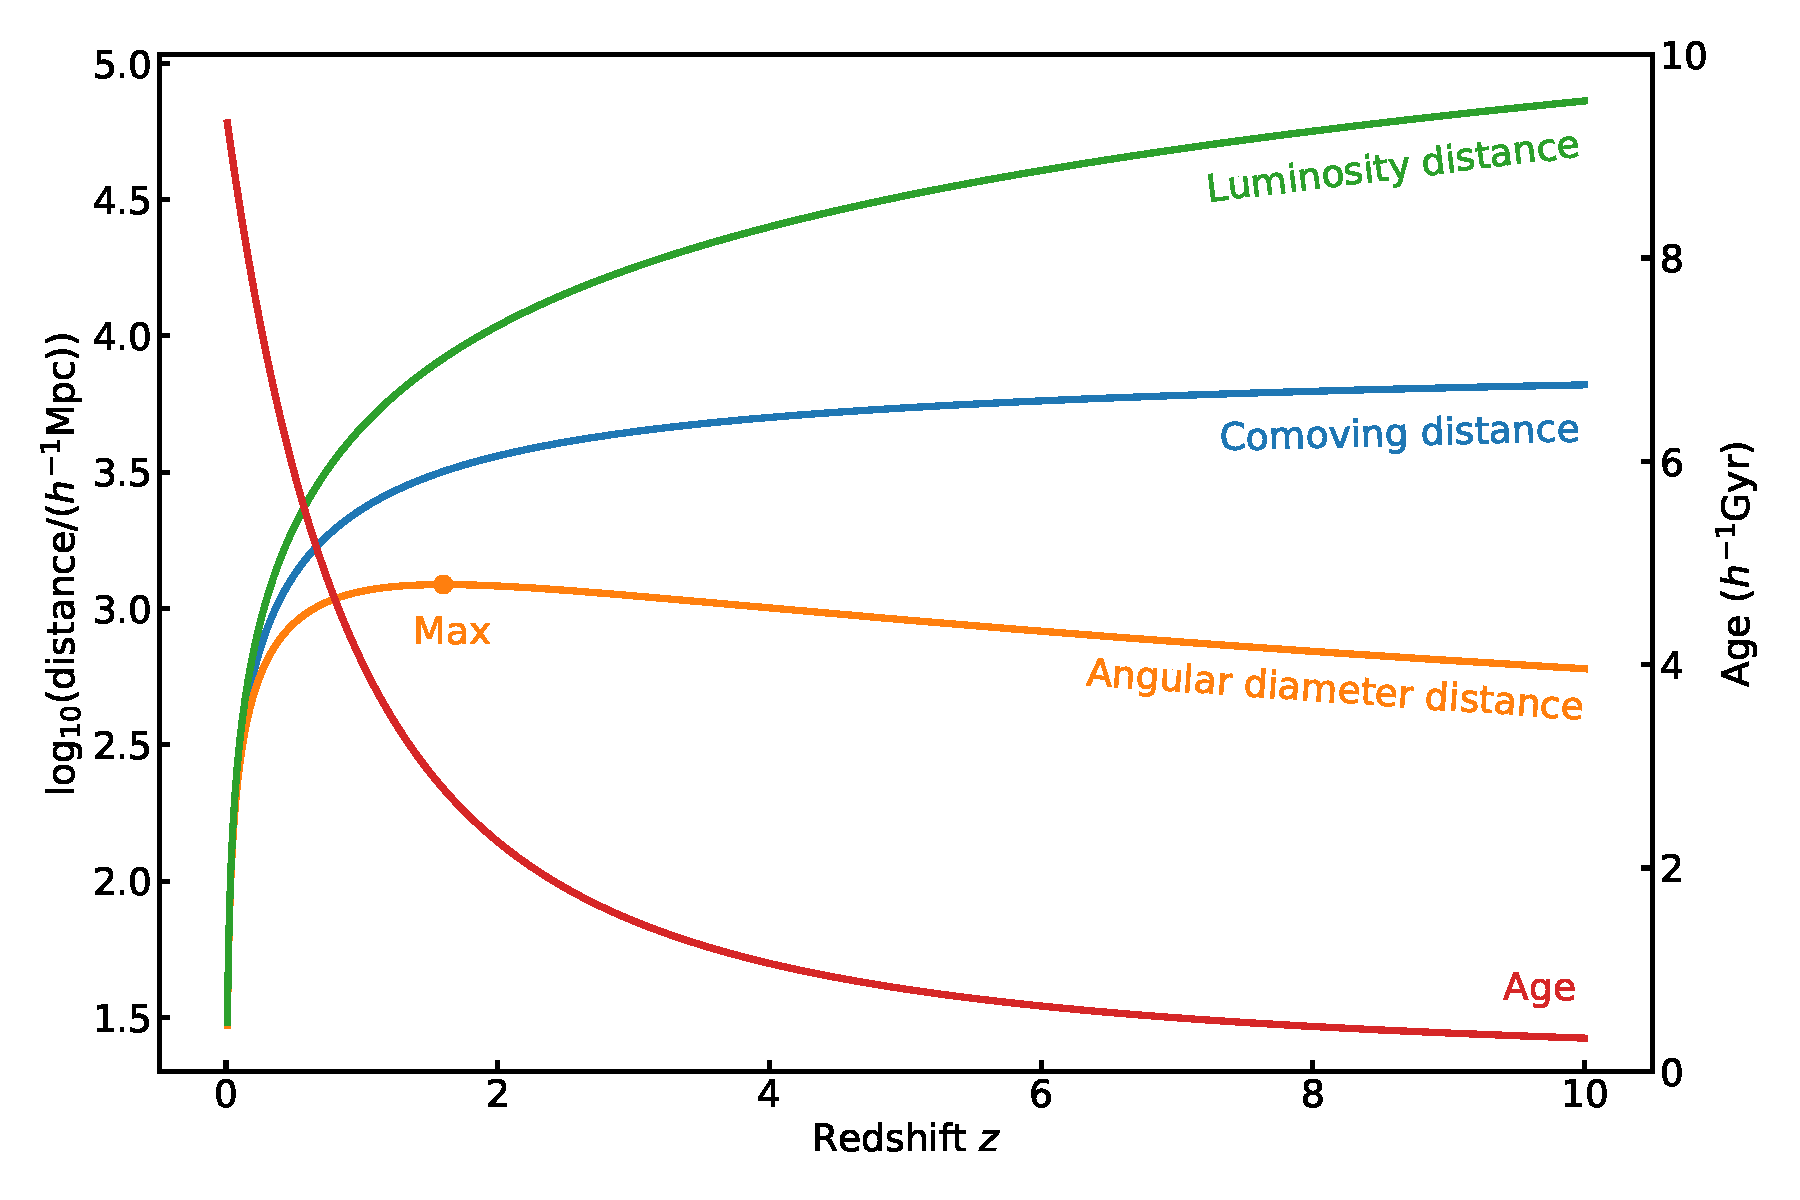
\includegraphics[width=0.9\textwidth]{q1_plot}
  \caption{Distances (left axis) and age (right axis) for a flat Universe with $\Omega_m=0.3$ and $\Omega_\Lambda=0.7$. The maximum value of the angular diameter distance $d_A$ occurs at $(z,d_A)=(1.61,1.22\,h^{-1}\mathrm{Gpc})$.}
  \label{fig:q1}
\end{figure}
\newpage
{\large {\bf Question 2}}

If stars are formed at redshift $z=4$, their age at $z=3$ is equal to the difference in the ages of the Universe at these two redshifts. Hence, denoting the stars' age as $\Delta t$:
\begin{align}
  \Delta t&=t(z\shorteq 3)-t(z\shorteq 4)\\
          &=418\,h^{-1}\mathrm{Myr}\nonumber
\end{align}

{\large {\bf Question 3}}

Lyman-$\alpha$ sources with rest-frame wavelength $\lambda_e=1215.67\,\mathrm{A\o}$ will be detected if their observed (redshifted) wavelength $\lambda_o$ falls within the range that the filter transmits. Hence the survey will collect light from objects distributed over a range of redshifts. Using $z=\lambda_o/\lambda_e-1$, this range is found to be $2.99<z<3.01$.

The physical size of the telescope field at these redshifts $\ell$ can be found using the angular diameter distance: 
\begin{equation}
  \ell(z)=\theta d_A(z)
  \label{eq:ellz}
\end{equation}

Evaluating \cref{eq:ellz} for the redshift range of the survey gives $\ell(z\shorteq 2.99)=1.621\,h^{-1}\mathrm{Mpc}$ and $\ell(z\shorteq 3.01)=1.617\,h^{-1}\mathrm{Mpc}$ respectively; as these values are similar their average may be treated as a constant value for $\ell$ over the redshift range considered.

The comoving and physical volumes are then found by multiplying $\ell^2$ by the corresponding value for the depth of the survey:
\begin{align}
  V_{\mathrm{comoving}}&=\ell^2\times\left(d_x(z\shorteq 3.01)-d_x(z\shorteq 2.99)\right)\label{eq:cmv}\\
  V_{\mathrm{physical}}&=\ell^2\times\left(d_r(z\shorteq 3.01)-d_r(z\shorteq 2.99)\right)\label{eq:phv}
\end{align}

where the physical distance $d_r$ is given by:
\begin{equation}
  d_r(z)=\frac{c}{H_0}\int_0^z\frac{\mathrm{d}z'}{(1+z')E(z')} 
\end{equation}

Evaluating \cref{eq:cmv,eq:phv} gives the results $V_{\mathrm{comoving}}=43.5\,h^{-3}\mathrm{Mpc}^3$ and $V_{\mathrm{physical}}=10.9\,h^{-3}\mathrm{Mpc}^3$.

To find the intrinsic surface brightness of a distant galaxy, the observed surface brightness in $\mathrm{mag/arcsec^2}$ first needs to be converted into physical units. Apparent magnitude is defined as:
\begin{equation}
  \label{eq:apmag}
  m_B=M_{\odot,B}-2.5\log_{10}(L_B)+5\log_{10}(d/10\mathrm{pc})
\end{equation}

where the $B$ subscript indicates magnitudes and luminosities in the corresponding band are considered (as this band overlaps with the wavelength of the filter).

The luminosity may be expressed as $L_B=(d\ \mathrm{arcsec})^2S_{\mathrm{phys}}$, where $S_{\mathrm{phys}}$ is the surface brightness in physical units of $L_{\odot,B}/\mathrm{pc}^2$. Substituting this into \cref{eq:apmag} gives:
\begin{equation}
  \label{eq:sbphys}
  \mu=M_{\odot,B}+21.572-2.5\log_{10}S_{\mathrm{phys}}
\end{equation}

where $\mu$ is the apparent surface brightness in magnitude units. Using $M_{\odot,B}=5.48$ and substituting the given $\mu=28$, \cref{eq:sbphys} may be rearranged to obtain $S_\mathrm{phys}=0.418\,L_{\odot,B}/\mathrm{pc^2}$.

From the notes:
\begin{equation}
  \label{eq:apsb}
  S_i=4\pi(1+z)^4S_a
\end{equation}

where $S_i$ and $S_a$ are respectively the intrinsic and apparent surface brightnesses in physical units. Taking $z=3$, \cref{eq:apsb} gives $S_i=1340\,L_{\odot,B}/\mathrm{pc^2}$.

Finally, \cref{eq:sbphys} may be used to convert this back into magnitude units, yielding the result: $$\mu=19.2\,\mathrm{mag/arcsec^2}$$

\end{document}